\documentclass[onecolumn]{article}
%\usepackage{url}
%\usepackage{algorithmic}
\usepackage[a4paper]{geometry}
\usepackage{datetime}
\usepackage[margin=2em, font=small,labelfont=it]{caption}
\usepackage{graphicx}
\usepackage{mathpazo} % use palatino
\usepackage[scaled]{helvet} % helvetica
\usepackage{microtype}
\usepackage{amsmath}
\usepackage{subfigure}
% Letterspacing macros
\newcommand{\spacecaps}[1]{\textls[200]{\MakeUppercase{#1}}}
\newcommand{\spacesc}[1]{\textls[50]{\textsc{\MakeLowercase{#1}}}}

\title{\spacecaps{Ceng 3521 Data Mining Final Project: Luad Lusc Cancer}\ 
\normalsize \spacesc }


\author{Osman Batuhan Şahin - Mehmet Cihan Sakman \\ osmanbatuhansahin@posta.mu.edu.tr - mehmetcihansakman@posta.mu.edu.tr\\github: \textbf{https://github.com/osmanbatuhansahin/final\_datamining}}
%\date{\today\\currenttime}
\date{\today}

\begin{document}
\maketitle

\begin{abstract}
In this project, we'll build Machine Learning algorithms to predict LUAD(Lung Adenocarcinoma)-LUSC(Lung squamous cell carcinoma) patient's risk level(high risk-low risk) based on dataset which obtained from TCGA dataset. During this project we'll commonly use \textbf{scikit-learn} library from Python. While applying Machine Learning Algorithms we'll build five different algorithms as: Support Vector Machine, Logistic Regression, Naive Bayes, Random Forest and K Neighbors classifiers.
\end{abstract}

\section{Introduction}
The main purpose of this project is predict Lung Cancer patient's risk level based on Machine Learning algorithms. Lung cancer is the most common and deadly cancer in the world. Each year more than one million people have diagnosed with lung cancer and the \%85 of them are Luad and Lusc cancer. We aim to build a Machine Learning algorithm to predict patient's risk levels for the prevention of incoming deaths because of lung cancer. 

List of important features for LUAD-LUSC dataset:
\begin{itemize}
    \item \emph{primary\_diagnosis} : patient's diagnosis more specifically
    \item  \emph{tumor\_stage} 
    \item  \emph{vital\_status} : patient is alive or dead
    \item  \emph{morphology} : The morphology code which describes the characteristics of the tumor itself, including its cell type and biologic activity, according to the third edition of the International Classification of Diseases for Oncology (ICD-O)
    \item  \emph{days\_to\_death} : How long patient live after diagnosed with lung cancer. No information for alive patients
    \item  \emph{days\_to\_birth} : age of the patient in days
    \item  \emph{cigarettes\_per\_day}
    \item  \emph{site\_of\_resection\_or\_biopsy} : which site of lung has damaged
    \item  \emph{years\_smoked}
    \item  \emph{gender}
    \item  \emph{race} 
    \item  \emph{ethnicity}
    \item  \emph{disease} : LUAD or LUSC
    \item  \emph{risk\_of\_patient}: high or low
     \item \emph{age\_at\_diagnosis} : old of patient when he/she diagnosed with lung cancer(in days)
\end{itemize}
\bigbreak
\section{Loading and Overview of Data}
We load our datasets as seen below. There were two csv files for LUAD and LUSC cancer patient's clinical information. There were no information about their risk of level and we load four oher csv files and concatenate them together.
\begin{figure}[h]
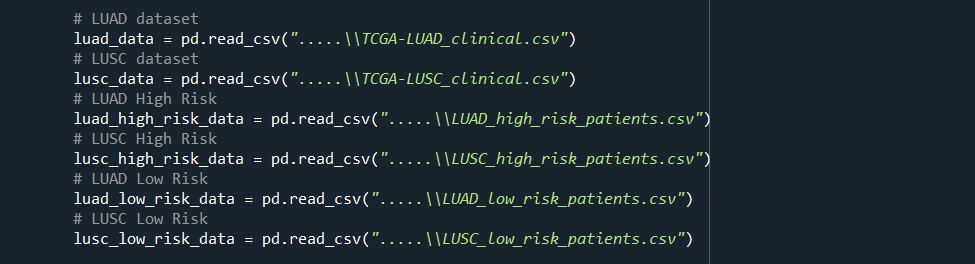
\includegraphics[scale=0.7]{load_dataset.png}
\caption{\emph{Loading Dataset}}
\centering
\end{figure}
\bigbreak

For the high risk and low risk csv files there were just one column which includes patient's ID and we add a new column into data which matches with these ID's.
\begin{figure}[h]
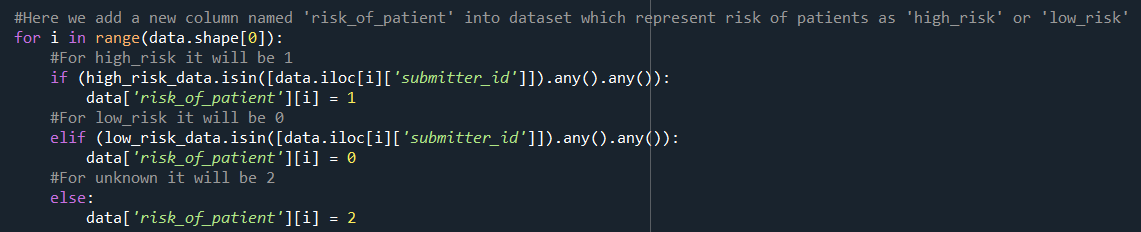
\includegraphics[scale=0.7]{risk_of_patient.png}
\caption{\emph{Loading Risk Levels of Patients}}
\centering
\end{figure}
\clearpage
Before pre-processing we can see how many columns and rows we have in our dataset and what are the column names.
\begin{figure}[h]
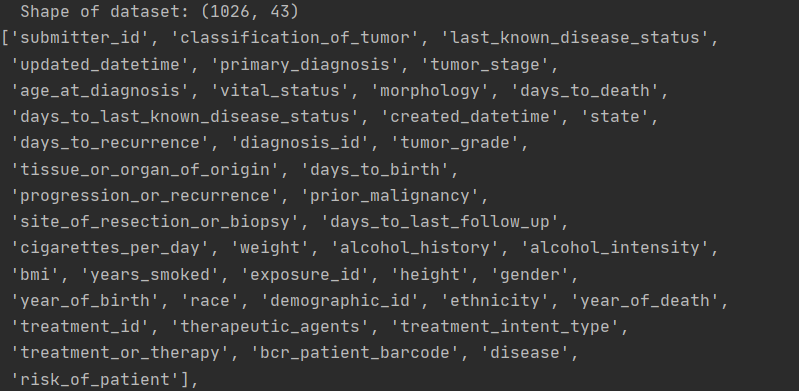
\includegraphics[scale=0.6]{shapee.png}
\caption{\emph{Shape of Dataset}}
\centering
\end{figure}

We can see how many missing values we have for each column.
\begin{figure}[h]
    \centering
    \begin{minipage}{0.4\textwidth}
        \centering
        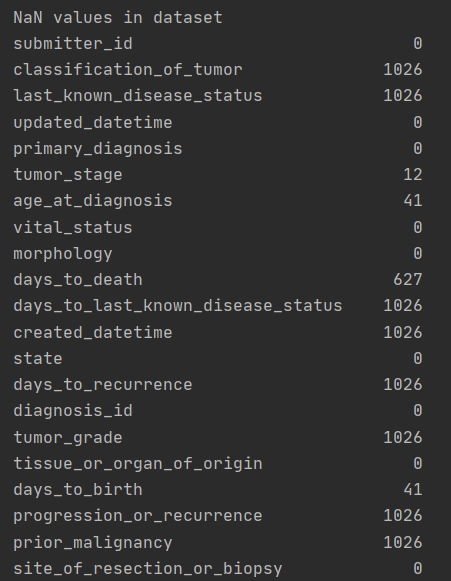
\includegraphics[width=1.0\textwidth]{nan1.png} % first figure itself
    \end{minipage}\hfill
    \begin{minipage}{0.4\textwidth}
        \centering
        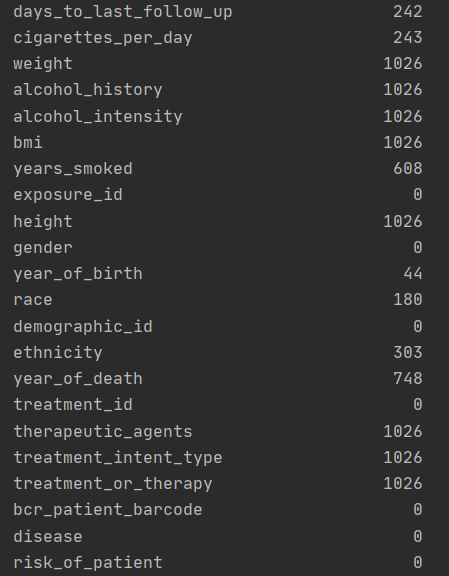
\includegraphics[width=1.0\textwidth]{nan2} % second figure itself
    \end{minipage}
    \bigbreak
    \caption{\emph{NaN values in dataset for each column}}
\end{figure}
\section{Preproccessing}
\subsection{Cleaning}

\subsubsection{Drop fully NaN Columns}
In our dataset(total patient 1026) we don't have any information about some features. As we can see in \emph{Figure 4} there are 16 features that are fully NaN.

\subsubsection{Drop IDs} % the star suppresses numbering of sections and subsections
There is no need to use ID columns for our learning algorithms because these are just random values for identifying specific objects. Therefore we dropped \emph{submitter\_id, diagnosis\_id, exposure\_id, demographic\_id, treatment\_id, bcr\_patient\_barcode} columns from dataset.

\subsubsection{Drop Useless Columns}
In our data there are some dummy and duplicate columns such as \emph{year\_of\_birth, state, updated\_datetime, tissue\_or\_organ\_of\_origin}. We don't need year\_of\_birth column because we can find the age of the patient from days\_to\_birth(in days) column. In \emph{state} feature, all the values are the same as \emph{'released'} therefore we can drop it. Also in updated\_datetime all the values are the same. Therese is duplicate columns that tissue\_or\_organ\_of\_origin and site\_of\_resection\_or\_biopsy and we dropped one of them.
\subsection{Dealing with Missing Values}
\subsubsection{Days to death Column}
In our days\_to\_death\_, there is just information about dead patients, and we expect to correlate that feature with the patient's vital status and patient risk level. For dealing with this problem we improve three different solutions:\\
\textbf{a)}Assign 0 for all alive patient and drop if there is such patient which is dead but it's days\_to\_death\_ value is 0. As we can see we have found 0.63 correlation with vital status but we couldn't find any correlation with risk of patient. \\
\textbf{b)}Assume that all the patients will live until 90 years old and fill the NaN values for alive patients assuming that they will live until their 90s. As we can see we have found 0.83 correlation with vital status but we couldn't find any correlation with risk of patient. \\
\textbf{c)}Also there is another feature called \emph{days\_to\_last\_follow\_up}. It's just the opposite of days\_to\_death\_ column. There is information about how long alive people have their check-in and there is no information about the dead patients. We just transfer the alive patient information into days\_to\_death\_ column and drop the days\_to\_last\_follow\_up column. As we can see we couldn't find any correlation for days to death neither between vital status nor risk of the patient.\\
In conclusion we decided to adopt second approach and we assume that all alive patient will live until their 90s.
\clearpage
\begin{figure}[h]
\caption{\emph{Heatmap correlations for approaches}}
    \centering
    \begin{minipage}{0.4\textwidth}
        \centering
        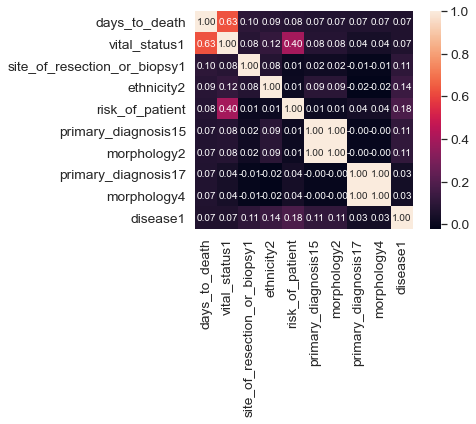
\includegraphics[width=1.0\textwidth]{sıfır.png} % first figure itself
        \emph{\small Filling with 0}\par\medskip
    \end{minipage}
    \begin{minipage}{0.4\textwidth}
        \centering
        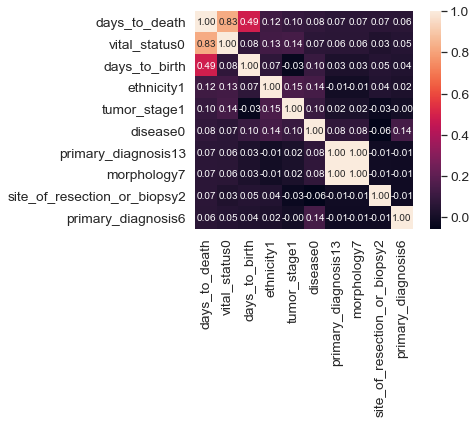
\includegraphics[width=1.0\textwidth]{90yas.png} % second figure itself
        \emph{\small Filling with days until 90s}\par\medskip
    \end{minipage}
    \bigbreak
    \begin{minipage}{0.4\textwidth}
        \centering
        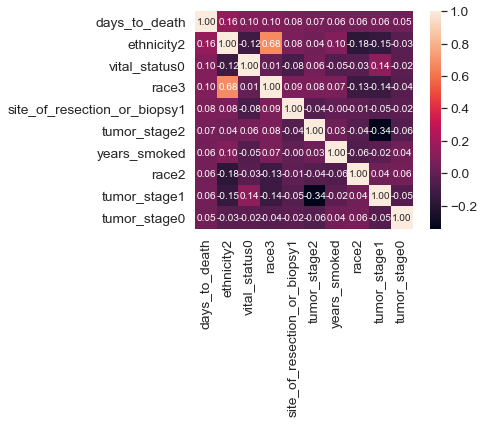
\includegraphics[width=1.0\textwidth]{days_to_follow_up.png} % first figure itself
        \emph{\small Filling with days\_to\_last\_follow\_up}\par\medskip
    \end{minipage}
\end{figure}

\subsubsection{Filling NaN values in Numeric Features with mean}
There are several approaches to dealing with missing values. One of them and the common one is filling these values with the mean value of the feature. There is a special library called \textbf{SimpleImputer} in \textbf{scikit-learn} to achieve this. Using this library with strategy \textbf{mean} we can fill the missing numerical values with the mean value of the feature. In our dataset we applied these approach for our \emph{"age\_at\_diagnosis", "days\_to\_birth", "cigarettes\_per\_day", "years\_smoked"} columns and filled the missing values.

\subsubsection{Dealing with missing values for \emph{ethnicity and race}}
We have 158 missing values for \emph{ethnicity} and 279 missing values for the \emph{race}. These two features are really important biologically because race and ethnicity may affect directly the cancer probability of a human. Therefore we didn't want to fill this column or drop them from the dataset because we didn't want to lose 279 patient information and we decided to keep the NaN values as \emph{'unknown'}.


\subsection{Encoding}
\subsubsection{OneHotEncoding}
In real-world data, categorical values may happen some problems for learning algorithms when we try to fit a machine learning model. Categorical data are variables that contain label values rather than numeric values. For instance, a \emph{“color”} variable with the values:\emph{“red“, “green” and “blue“}. Each value represents a different category. The main problem with categorical data is that many machine learning algorithms cannot operate on label data directly. They require all input variables and output variables to be numeric. Therefore we should encode our categorical data into numeric data. For achieve that there is a library in \textbf{scikit-learn} called \textbf{preprocessing}. For the first step, we should apply \textbf{LabelEncoder} to categorize each unique values into an integer value. After that, \emph{OneHotEncoding} can be applied to the integer representation. This is where the integer encoded variable is removed and a new binary variable is added for each unique integer value.
We apply this approach for all our categorical values. There is an example to see it better.

\begin{figure}[h]
    \centering
    \begin{minipage}{0.4\textwidth}
        \centering
        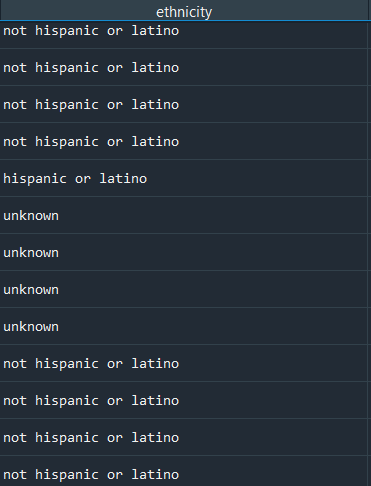
\includegraphics[width=1.42\textwidth]{before_encoding.png} % first figure itself
    \end{minipage}\hfill
    \begin{minipage}{0.39\textwidth}
        \centering
        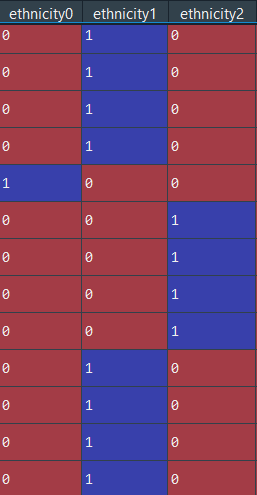
\includegraphics[width=1.0\textwidth]{after_encoding.png} % second figure itself
    \end{minipage}
    \bigbreak
    \caption{\emph{OneHotEncoding}}
\end{figure}

\subsection{Scaling Problem}
We didn't apply any scaling algorithm to our Machine Learning algorithms because scaling has negative effects on our learning algorithm. Due to we are working with biological data we avoided the scaling data.

\subsection{Summary of Preprocessing}
At the end of the pre-processing we clean up our data from dummy variables, duplicate features, and NaN values, and using \emph{OneHotEncoder} we transformed the categorical values into unique columns. After all this operations now we have \emph{965} rows and \emph{72} columns and there is no NaN values in data.
\begin{figure}[h]
    \centering
    \begin{minipage}{0.4\textwidth}
        \emph{\small Shape of Data and Columns}\par\medskip
        \centering
        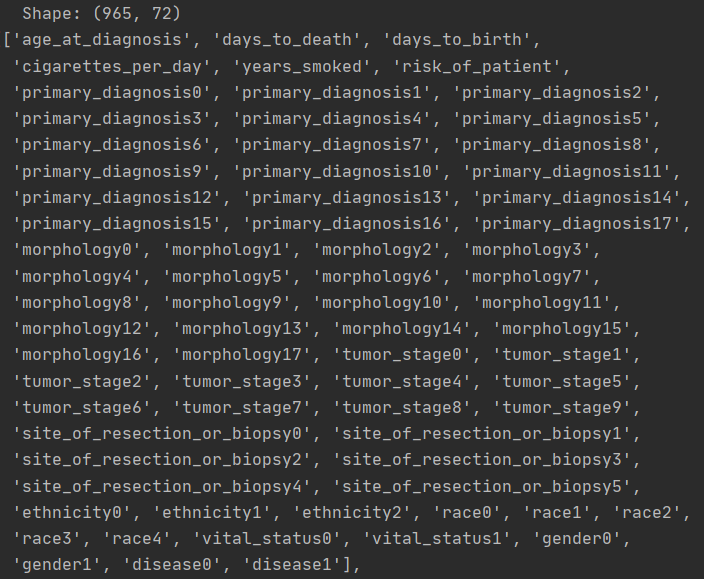
\includegraphics[width=1.2\textwidth]{endofpreprocess.png} % first figure itself
    \end{minipage}\hfill
    \begin{minipage}{0.4\textwidth}
        \emph{\small Non Null Values}\par\medskip
        \centering
        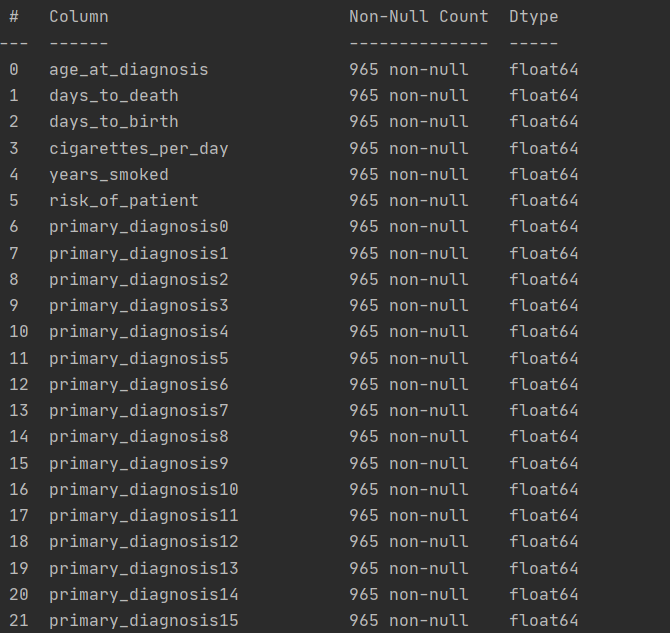
\includegraphics[width=1.0\textwidth]{afterpreprocessnotnull.png} % second figure itself
    \end{minipage}
    \bigbreak
    \caption{\emph{End of Preprocessing}}
\end{figure}

\subsection{Splitting Data}
We splitted our data such that randomly selected \%80 tuples are used for training while \%20 tuples are used for testing with \textbf{train\_test\_split} from \textbf{sklearn} library.


\section{Apply Machine Learning Algorithms}
After preprocessing we prepared our dataset for applying learning algorithms. We wanted to build five different learning algorithms to find the best for our dataset. We will use the following algorithms: Support Vector Machine, Logistic Regression, Naive Bayes, Random Forest, and K Neighbors Classifiers. Our aim to use these algorithms is that predicting the risk levels of our lung cancer patients whether they are high-risk level or low-risk level. Before these predictions, we can plot the importance of features.
\begin{figure}[h]
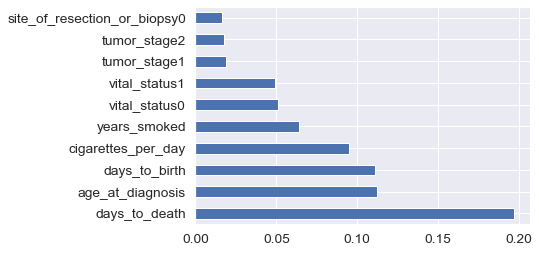
\includegraphics[scale=0.7]{importancee.png}
\caption{\emph{Importance of 10 Features}}
\centering
\end{figure}
\subsection{Support Vector Machine Algoirthm}
Support vector machine is highly preferred by many as it produces significant accuracy with less computation power. Support Vector Machine, abbreviated as SVM can be used for both regression and classification tasks. But, it is widely used in classification objectives and we also wanted to use this classification algorithm in our dataset. After fitted our dataset into Support Vector Machine algorithm and predict the ground truth vector with \%69.43 accuracy score.
\begin{figure}[h]
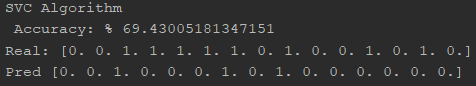
\includegraphics[width=15cm, height=2cm]{SVC_score.png}
\caption{\emph{SVC Score}}
\centering
\end{figure}

\subsection{Logistic Regression Algoirthm}
Logistic Regression is the most common learning algorithm for classification tasks. Due to our ground truth vector is binary Logist Regression is on of the best option for our data. After fitted our dataset into Logistic Regression algorithm and predicted the ground truth vector with \%67.87 accuracy score.
\begin{figure}[h]
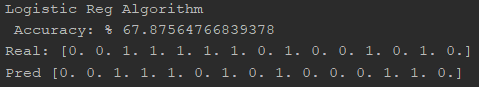
\includegraphics[width=15cm, height=2cm]{Logistic.png}
\caption{\emph{Logistic Regression Score}}
\centering
\end{figure}
\subsection{Naive Bayes Algoirthm}
Naive Bayes is a classification technique based on Bayes’ Theorem with an assumption of independence among predictors. In simple terms, a Naive Bayes classifier assumes that the presence of a particular feature in a class is unrelated to the presence of any other feature. After fitted our dataset into Naive Bayes algorithm and predicted the ground truth vector with \%67.87 accuracy score.
\begin{figure}[h]
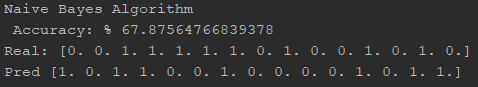
\includegraphics[width=15cm, height=2cm]{NaiveBayes.png}
\caption{\emph{Naive Bayes Score}}
\centering
\end{figure}
\subsection{Random Forest Algoirthm}
Random forests is a supervised learning algorithm. It can be used both for classification and regression. It is also the most flexible and easy to use algorithm. A forest is comprised of trees. It is said that the more trees it has, the more robust a forest is. Random forests creates decision trees on randomly selected data samples, gets prediction from each tree and selects the best solution by means of voting. After fitted our dataset into Random Forest algorithm and predicted the ground truth vector with \%62.17 accuracy score. Also for improve Random Forest algorithm we try to find best \emph{n\_estimators}.
\begin{figure}[h]
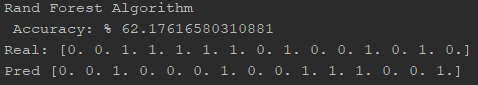
\includegraphics[width=15cm, height=2cm]{RandForest.png}
\caption{\emph{Random Forest Score}}
\centering
\end{figure}
\subsection{K Neighbors Classifiers Algoirthm}
K nearest neighbors is a simple algorithm that stores all available cases and classifies new cases based on a similarity measure (e.g., distance functions). A case is classified by a majority vote of its neighbors, with the case being assigned to the class most common amongst its K nearest neighbors measured by a distance function. If K = 1, then the case is simply assigned to the class of its nearest neighbor. With random parameter settings we fitted our dataset into KNN algorithm and predicted the ground truth vector with \%67.87 accuracy score. Also for improve KNN algorithm we try to find best \emph{n\_neighbors}.
\clearpage
\begin{figure}[h]
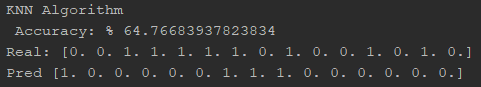
\includegraphics[width=15cm, height=2cm]{KNN.png}
\caption{\emph{KNN Score}}
\centering
\end{figure}

\subsection{Best Parameters for KNN and Random Forest}
For improving accuracy scores we try to find best parameters for KNN and Random Forest. In conlusion of these operation we found that the best \emnph{n\_estimators} for \textbf{Random Forest} is 25 with \%70.9 accuracy score and the best \emph{n\_neighbors} for \textbf{KNN} is 18 with \%71.5 accuracy score.
\begin{figure}[h]
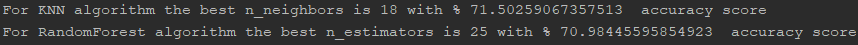
\includegraphics[width=15cm, height=2cm]{improve.png}
\caption{\emph{Improvement Scores}}
\centering
\end{figure}
\subsection{Apply Machine Learning Algoirthms with PCA}
Principal Component Analysis (PCA) is an unsupervised, non-parametric statistical technique primarily used for dimensionality reduction in machine learning. To improve our accuracy scores we try to reduce our dimensionality with parameters (10,20,30,40,50,60). You can find the results below.
\begin{figure}[h]
    \centering
    \begin{minipage}{0.4\textwidth}
        \centering
        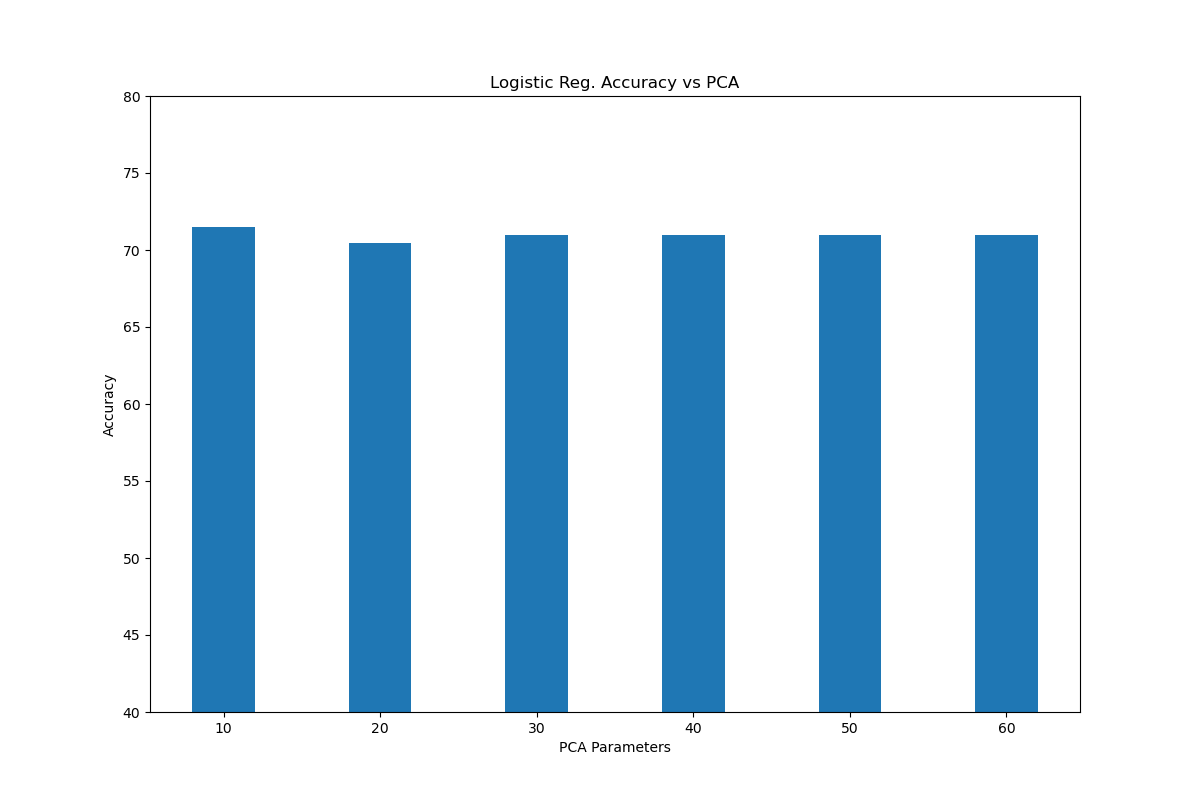
\includegraphics[width=1.3\textwidth]{pca_logistic.png} % first figure itself
    \end{minipage}\hfill
    \begin{minipage}{0.4\textwidth}
        \centering
        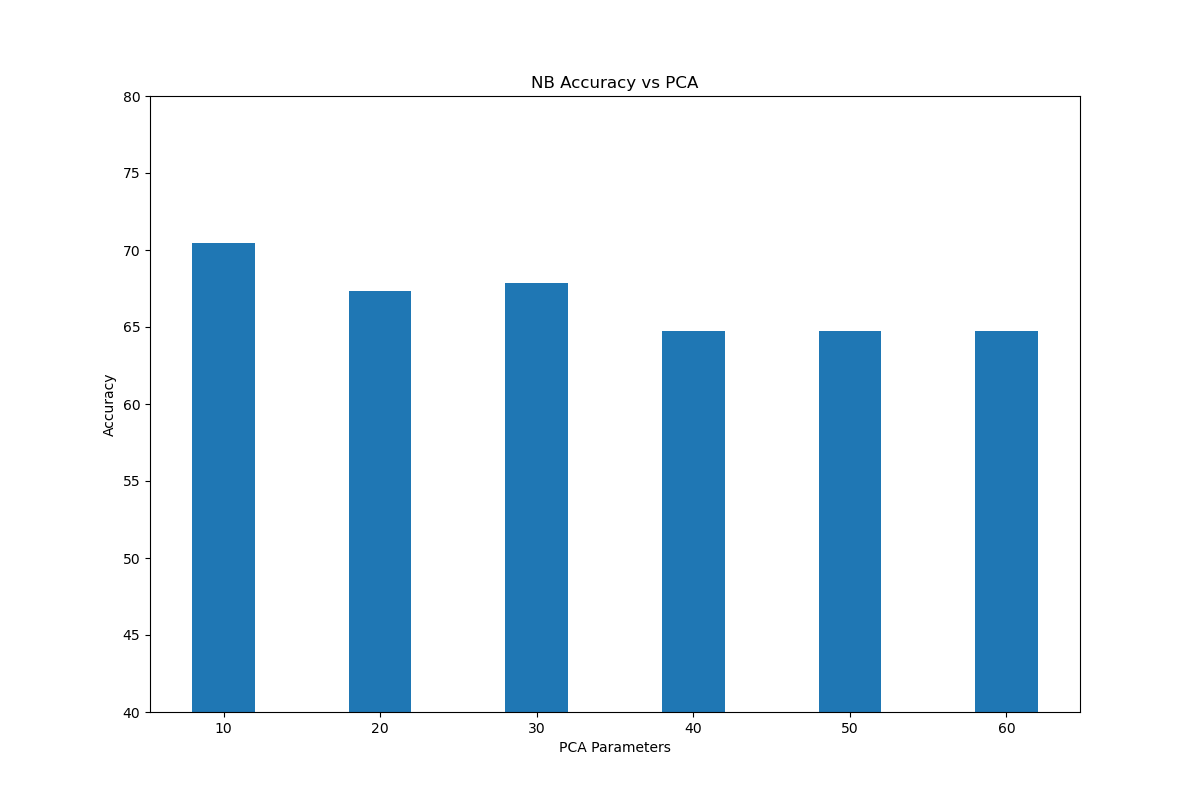
\includegraphics[width=1.3\textwidth]{pca_NaiveBayes.png} % second figure itself
    \end{minipage}
    \bigbreak
\end{figure}
\clearpage
\begin{figure}[h]
    \centering
    \begin{minipage}{0.4\textwidth}
        \centering
        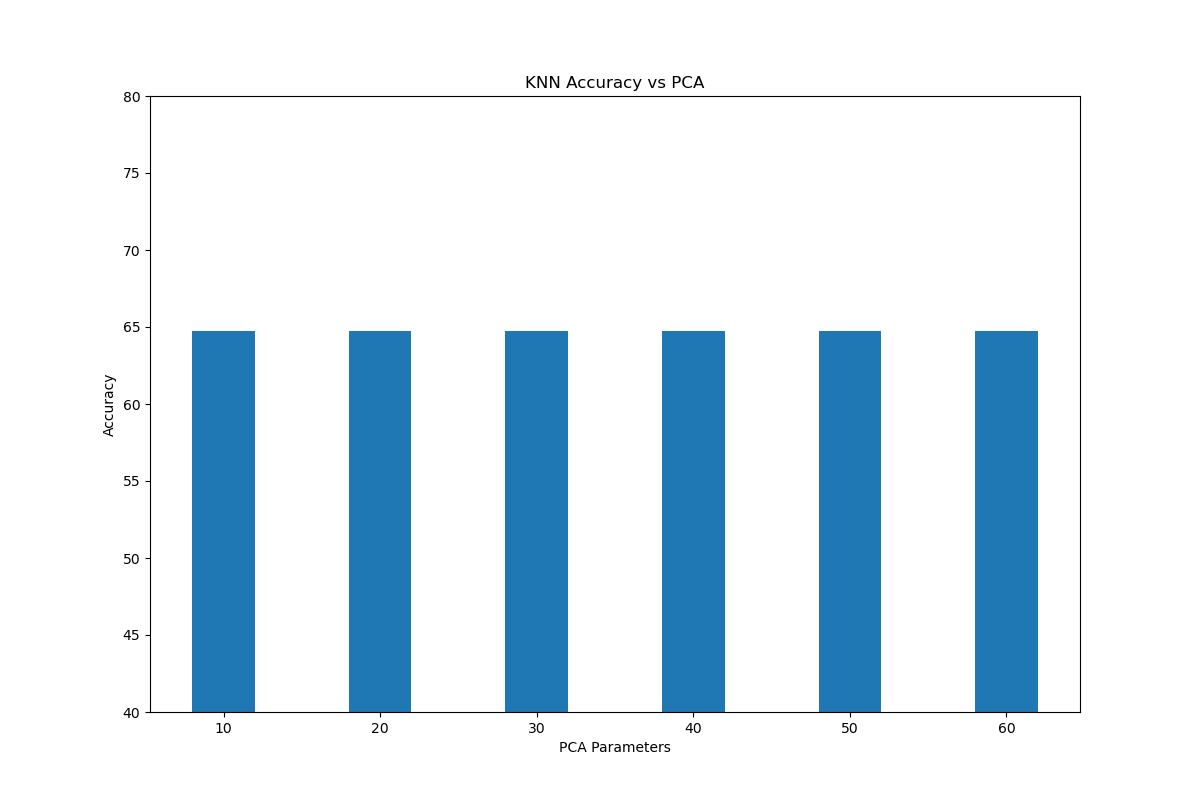
\includegraphics[width=1.3\textwidth]{pca_KNN.png} % first figure itself
    \end{minipage}
    \begin{minipage}{0.4\textwidth}
        \centering
        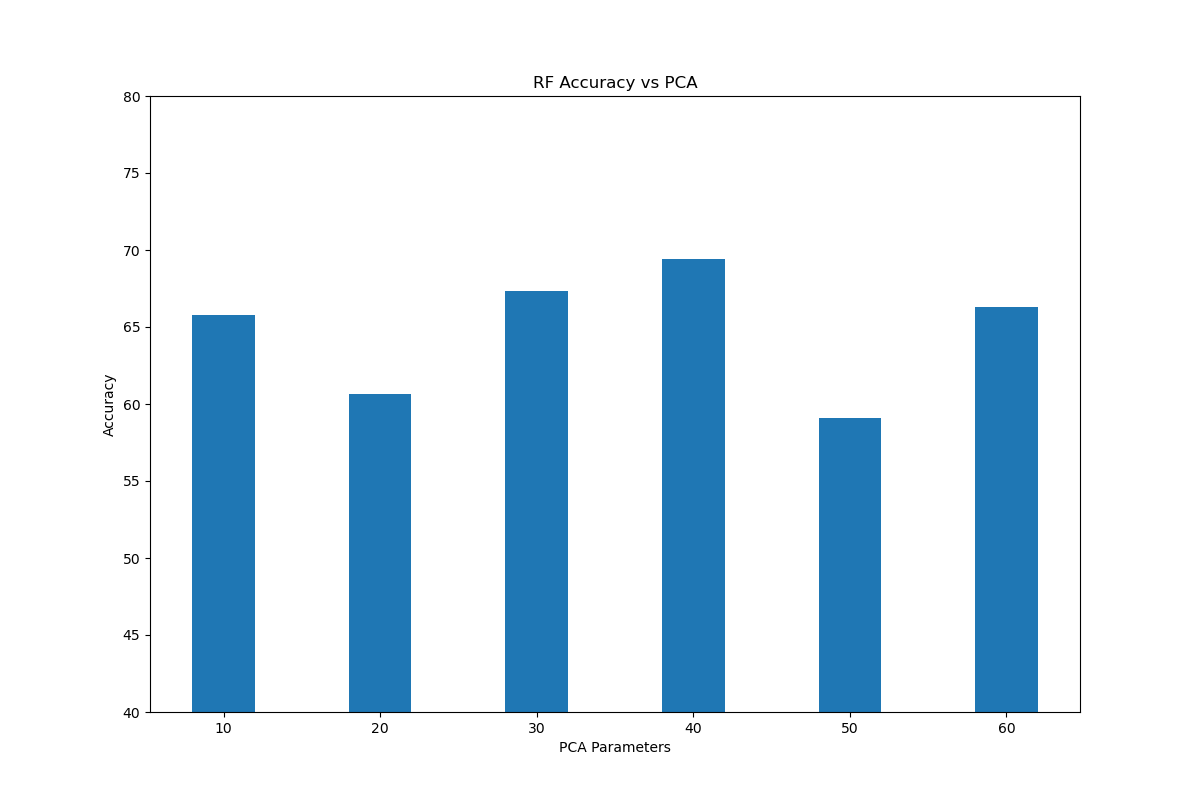
\includegraphics[width=1.3\textwidth]{pca_RF.png} % second figure itself
    \end{minipage}
    \bigbreak
    \begin{minipage}{0.4\textwidth}
        \centering
        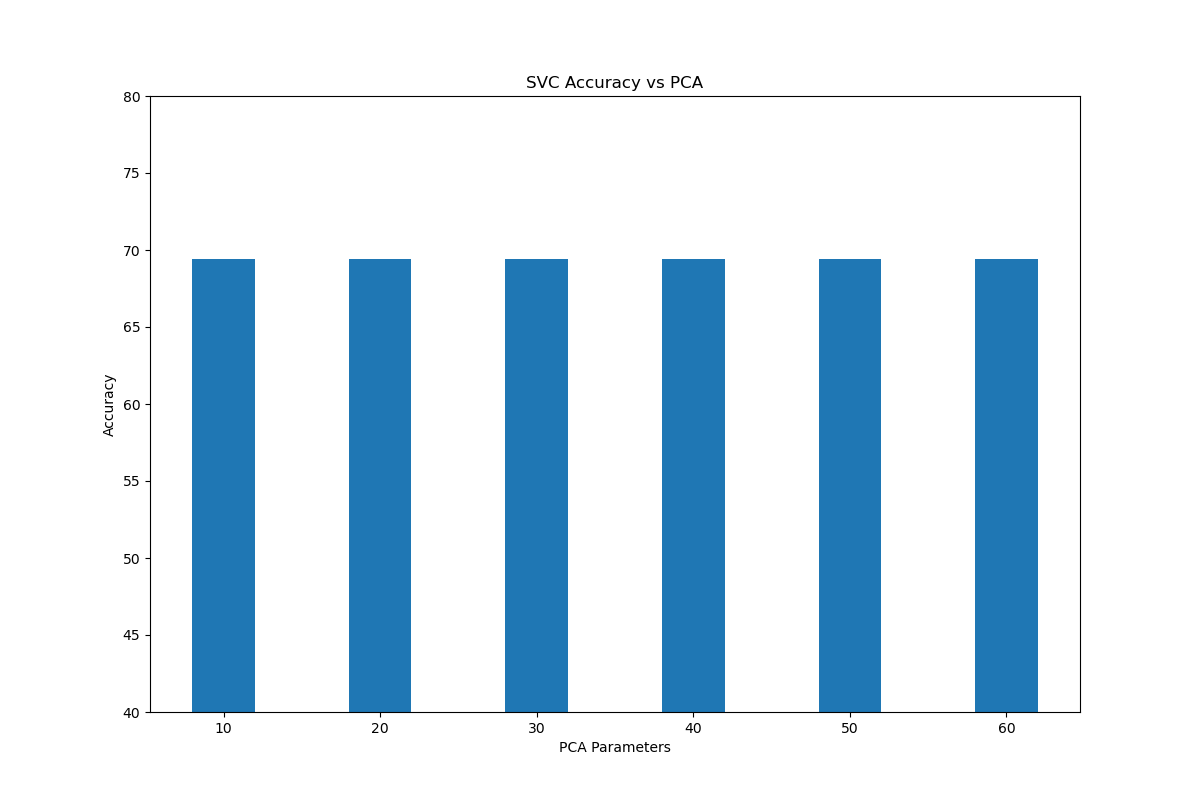
\includegraphics[width=1.3\textwidth]{pca_SVC.png} % first figure itself
    \end{minipage}
\end{figure}

\subsection{Comparision of Accuracy Scores}
In below figure we can better see which learning algorithm is better for default parameters.
\clearpage
\begin{figure}[h]
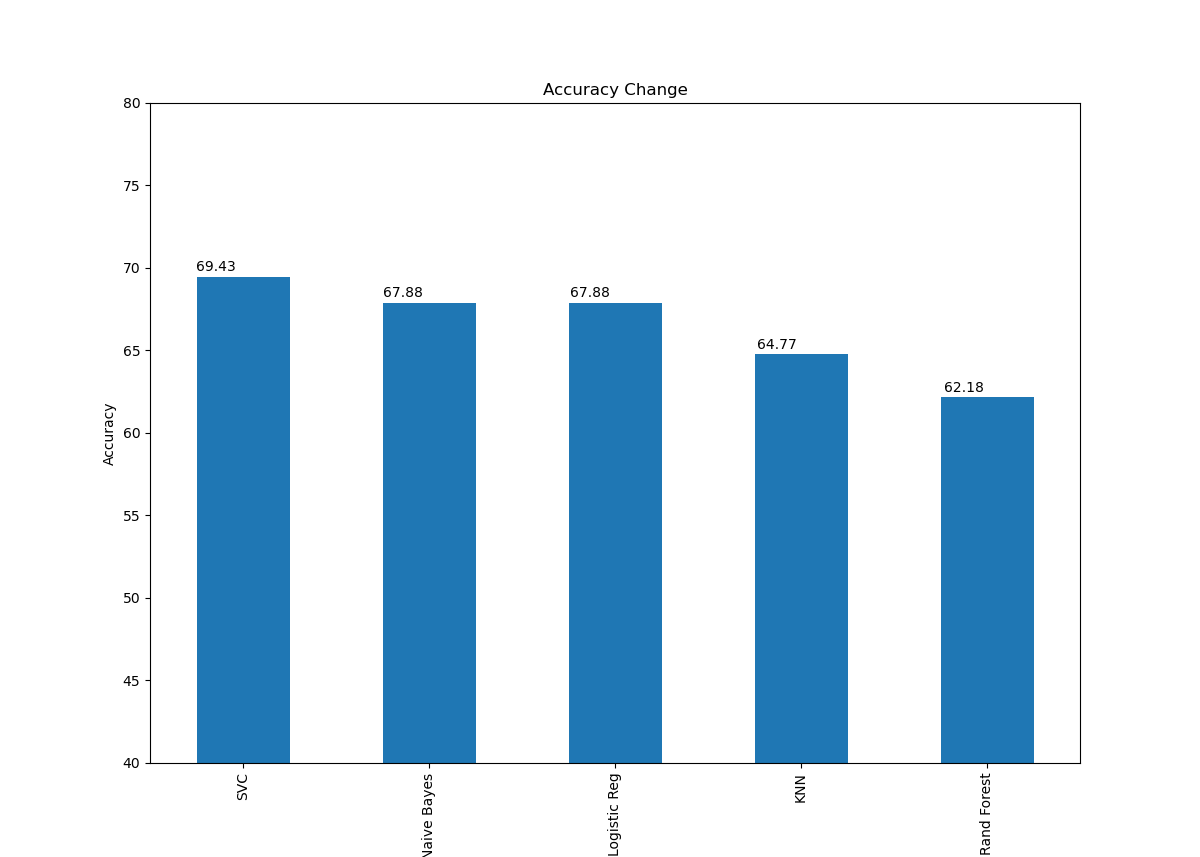
\includegraphics[width=15cm, height=10cm]{AccuracyChange.png}
\caption{\emph{SVC Score}}
\centering
\end{figure}

\section{Conclusion}
In conclusion, we tried to deal with LUAD and LUSC cancer patients and make a prediction about their risk levels. Due to this is a real-world problem our dataset was dirty and we had to clean up the data in preprocessing section. We dropped fully NaN, duplicate, and dummy features from our dataset. After that, we tried to fill NaN values with different approaches. At the end of the preprocessing, we applied OneHotEncoding to transforming categorical values into numeric values.
After preparing our dataset we applied five different classification algorithms to find the best algorithm for our dataset. After applying all algorithms we could not achieve as good results as we wanted. For improving our accuracy scores we applied the PCA algorithm to reduce dimension and have better accuracy scores. We can also clearly see in the figures we gained more than \%70 accuracy score for Logistic Regression with applying PCA algorithm. 
On the other hand with random parameters, KNN algorithm had \%64.8 accuracy score but after finding the best n\_neighbour parameter as 18 we gained \%71.5 accuracy score. Also for the Random Forest algorithm, we had \%62.5 accuracy score with random parameters but with the best n\_estimaters as 25, we gained \%70.9 accuracy score.
As a result, we conclude that for this learning algorithm KNN had the best accuracy score with the best parameter settings.



\nocite{*}
\bibliographystyle{plain}
\bibliography{references}
\end{document}